\documentclass[final,oneside,onecolumn,12pt,a4paper]{book}%
%薛丞宏加的
\usepackage{fontspec} 
\usepackage{xeCJK} 
\usepackage{ruby}
\XeTeXlinebreaklocale "zh" 
\XeTeXlinebreakskip = 0pt plus 1pt 
\renewcommand{\rubysep}{-4ex}
\pagestyle{empty}
%Select fonts
%\setmainfont[Mapping=tex-text]{Times New Roman} % rm
%\setsansfont[Mapping=tex-text]{Arial}           % sf
%\setmonofont{Courier New}                       % tt
\setCJKmainfont{DFKai-SB} %xelatex 標楷體
\setCJKmonofont{MingLiU}  %xelatex 細明體
\linespread{3}

\makeatletter
\newcommand{\rubybot}[2]{%
  \@tempdimc \f@size\p@
  \begin{tabular}[t]{@{}c@{}}
    #1\\[-3em]
    \fontsize{.8\@tempdimc}{.8\@tempdimc}\selectfont%
    \setlength{\normalbaselineskip}{0pt}#2 
  \end{tabular}%
}
\makeatother
\usepackage[toc,page]{appendix}
%薛丞宏加的

\usepackage{amsmath}
\usepackage{amsfonts}
\usepackage{amssymb}
\usepackage{url}
\usepackage{algorithm}
\usepackage{algorithmic}
\usepackage{graphicx}%
\setcounter{MaxMatrixCols}{30}
\usepackage[left=3cm, right=2cm, top=2.5cm, bottom=2.5cm]{geometry}
%TCIDATA{OutputFilter=latex2.dll}
%TCIDATA{Version=5.50.0.2953}
%TCIDATA{Created=Monday, May 12, 2003 22:46:51}
%TCIDATA{LastRevised=Friday, August 30, 2013 14:39:59}
%TCIDATA{<META NAME="GraphicsSave" CONTENT="32">}
%TCIDATA{<META NAME="SaveForMode" CONTENT="1">}
%TCIDATA{BibliographyScheme=BibTeX}
%TCIDATA{<META NAME="DocumentShell" CONTENT="Standard LaTeX\Blank - Standard LaTeX Article">}
%TCIDATA{Language=American English}
%TCIDATA{PageSetup=72,72,72,72,0}
%TCIDATA{Counters=arabic,1}
%TCIDATA{AllPages=
%H=36
%F=36
%}
%BeginMSIPreambleData
\providecommand{\U}[1]{\protect\rule{.1in}{.1in}}
%EndMSIPreambleData
\oddsidemargin 0.0in
\textheight=8.5in
\textwidth=6.5in
\headheight=0.0in
\topmargin=0.0in
\newtheorem{theorem}{Theorem}
\newtheorem{abstract}{abstract}
\newtheorem{acknowledgement}[theorem]{Acknowledgement}
\newtheorem{axiom}[theorem]{Axiom}
\newtheorem{case}[theorem]{Case}
\newtheorem{claim}[theorem]{Claim}
\newtheorem{conclusion}[theorem]{Conclusion}
\newtheorem{condition}[theorem]{Condition}
\newtheorem{conjecture}[theorem]{Conjecture}
\newtheorem{corollary}[theorem]{Corollary}
\newtheorem{criterion}[theorem]{Criterion}
\newtheorem{definition}[theorem]{Definition}
\newtheorem{example}[theorem]{Example}
\newtheorem{exercise}[theorem]{Exercise}
\newtheorem{lemma}[theorem]{Lemma}
\newtheorem{notation}[theorem]{Notation}
\newtheorem{problem}[theorem]{Problem}
\newtheorem{proposition}[theorem]{Proposition}
\newtheorem{remark}[theorem]{Remark}
\newtheorem{solution}[theorem]{Solution}
\newtheorem{summary}[theorem]{Summary}
\interdisplaylinepenalty=2500
\sloppy
\pagenumbering{arabic}
\pagestyle{plain}
\renewcommand{\baselinestretch}{2}
\begin{document}

\frontmatter
\chapter{踏頭話}
勞力~~
\newpage

\chapter{摘要}
謝謝

\newpage

\chapter{Abstract}

Thank you

\newpage

\tableofcontents
\listoffigures
\listoftables



\mainmatter


\chapter{研究背景}
\label{章:研究背景}

\rubybot{臺 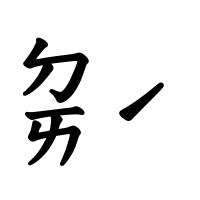
\includegraphics[height=1em]{圖/⿳⿳ㄉㄞˊ}}{tai5}
\rubybot{語 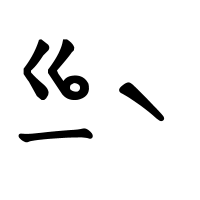
\includegraphics[height=1em]{圖/⿳⿳ㆣㄧˋ}}{gi2}

\section{臺語介紹}
\label{章:臺語介紹}

\section{語料狀況}
\label{節:語料狀況}

The rest of this paper is organized as follows. Chapter
\ref{章:相關研究} covers some preliminaries.
The three versions of the PTI discovery problem are formulated in Chapter
\ref{章:臺語介紹}. Chapter \ref{章:翻譯語料} presents our
solutions based on the shockwave approach. Our field trial and simulation
results are provided in Chapter \ref{章:摻猶未整理語料} and
\ref{章:網路語料庫}. Conclusions and future works are drawn in Chapter
\ref{章:結論佮未來發展}.

\chapter{相關研究}
\label{章:相關研究}


\chapter{翻譯語料}
\label{章:翻譯語料}

頂一章有講

\section{翻譯架構}
\label{節:翻譯架構}
國語翻譯到臺語需要兩項物件,一項是國語翻譯到臺語的語詞對照表,另外一項是知影臺語逐句好歹的語言模型。這馬時行的翻譯系統是統計翻譯(),會當分做三个部份:第一个是對齊模型(alignment model),負責產生語詞對照表,伊的做法是:第二部份是語言模型(),…。上尾一部份是解碼器(),用有效率的演算法來翻譯國語到臺語。
\section{評分方式}
\label{節:評分方式}

\section{新聞語料庫}
\label{節:新聞語料庫}

\section{未知詞問題}
\label{節:未知詞問題}

\section{改變語料格式}
\label{節:改變語料格式}

\section{未知詞另外翻譯}
\label{節:未知詞另外翻譯}

\chapter{摻猶未整理語料}
\label{章:摻猶未整理語料}
對於定定百萬句的翻譯來講傷少
加入其他的語料
教育部語料
數位典藏
 語料之間的問題
用字無一致
毋是一對一
斷詞方法無一致

\section{教育部語料佮數位典藏}
\label{節:教育部語料佮數位典藏}

\section{漢羅全羅對齊}
\label{節:漢羅全羅對齊}

\section{斷詞方法}
\label{節:斷詞方法}

\section{實驗流程佮結果}
\label{節:實驗流程佮結果}


\chapter{網路語料庫}
\label{章:網路語料庫}
現況
\section{TGB通訊-臺灣組合}
\label{節:TGB通訊-臺灣組合}

\section{語言判斷}
\label{節:語言判斷}

\section{實驗結果}
\label{節:實驗結果}


\chapter{結論佮未來發展}
\label{章:結論佮未來發展}

\chapter{--其他--}
To find $T$, we try to approximate a (real-value) GCD of $D=\left\{
T_{1},T_{2},...,T_{n-1}\right\}  $. This is done by running the DBSCAN
(Density Based Spatial Clustering of Applications with Noise) clustering
algorithm \cite{Ester1996DBSCAN} to group data items and filter out noise,
followed by a testing process to find $T$. There are several parameters used
in this approach:

In the simulations, VISSIM \cite{Mosseri2004VISSIM} was used to simulate
vehicle traffic. The Poisson arrival model with rates 18/20/24 vehicles per
minute was used to generate traffic flows into a signalized road section of
$650$ m from A to B as illustrated in Fig. \ref{fig:f_map} for $40$ minutes,
and the Wiedemann 99 car following model \cite{Mosseri2004VISSIM} was used to
depict the trajectories of vehicles. In the free flow state, vehicles move in
a range of speed between $48$ km/h and $58$ km/h. When encountering a red
signal, vehicles slow down and eventually stop. After the signal turned to
green, vehicles accelerate and then enter the free flow state.
\begin{figure}[pth]
\centerline{\includegraphics[angle=0, width=3.5in,keepaspectratio,clip]
{figures/f_map.eps}} \hfill\caption{The road segment in simulation and field
trial experiments. B is the location of the traffic light.}%
\label{fig:f_map}%
\end{figure}

\bibliographystyle{IEEEtran}
\bibliography{翻譯論文}

\begin{appendices}
\chapter{Some Appendix}
\chapter{Some Appendix}
The contents...
\end{appendices}

\end{document}